%%%%%%%%%%%%%%%%%%%% BlackSheep.tex %%%%%%%%%%%%%%%%%%%%%%%%


% Packages %%%%%%%%%%%%%%%%%%%%%%%%%%%%%%%%%%%%%%%%%%%%%%%%%%%
\documentclass[graybox]{svmult}

\usepackage{mathptmx}      
\usepackage{helvet}        
\usepackage{courier}       
\usepackage{type1cm}       
\usepackage{amsfonts}
\usepackage{makeidx}       
\usepackage{graphics}  
\usepackage{graphicx}     
\usepackage{subfigure}  

\usepackage{multicol}       
\usepackage[bottom]{footmisc}

\makeindex 

% New Commands
\newcommand{\PathSet}{\ensuremath{\mathcal P} }
\newcommand{\PathSetDistance}{\ensuremath{\mathcal G} }
\newcommand{\Z}{\mathbb{Z} }
\newcommand{\Path}{\ensuremath{P} }
\newcommand{\DCS}{\ensuremath{\Omega} }
\newcommand{\SetDistance}{\textsl{D} }
\newcommand{\PathDistance}{\textsl{PD} }

% Title %%%%%%%%%%%%%%%%%%%%%%%%%%%%%%%%%%%%%%%%%%%%%%%%%%%%%%%%

\begin{document}

\title*{Bounded Diverse Paths and their application in Path Planning}
\author{Ana Huam\'an Quispe and Mike Stilman}
\institute{Center for Robotics and Intelligent Machines, Georgia Institute of Technology,Atlanta GA,\\ \email{ahuaman3@gatech.edu, mstilman@cc.gatech.edu}}

\maketitle

% Abstract %%%%%%%%%%%%%%%%%%%%%%%%%%%%%%%%%%%%%%%%%%%%%%%%%%%%%%%

\abstract{We present a formal definition of Bounded Diverse Paths and how this approach can be applied in Path Planning.\newline\indent
Our approach rests on principles of Digital Imagery as well as Optimal Control. We show its application to a practical problem, such as how to find diverse paths.}

%%%%%%%%%%%%%%%%%%%%%%%%%%%%%%%%%%%%%%%%%%%%%%%%%%%%%%%%%%%%%%%%
% Introduction
\section{Introduction}
\label{sec:Introduction}
Motion planning problems usually involve computing collision-free paths from a start to a goal position. Great efforts have been focused in developing techniques to produce an \emph{optimal path}, according to some cost metric. While this is useful in some scenarios, it is also true that there are situations in which it would be more useful to produce more than one possible path as a solution. We illustrate this better as an example:

Assume that you have a robotic arm such as in Fig.\ref{fig:IntroductionStartPosition} and want to devise a path to reach the goal position in Fig.\ref{fig:IntroductionTargetPosition}. We decide to solve it by using Search-based techniques for high-dimensional spaces, such as \cite{}, \cite{}, which make use of a workspace heuristic to guide the configuration space search. 

\begin{figure}[]
		\centering
		  \subfigure[Start Position]{
		   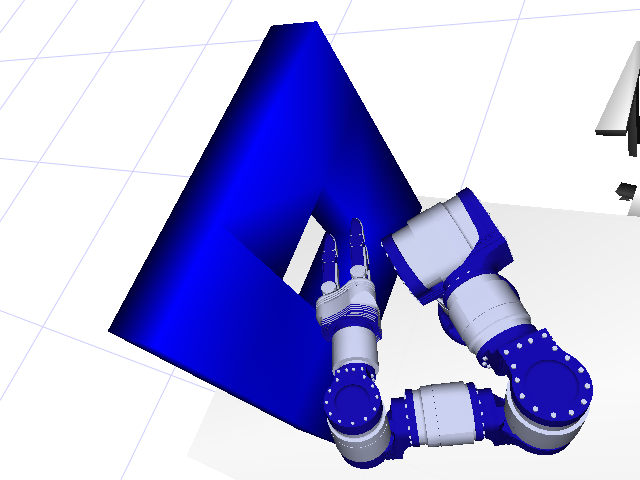
\includegraphics[width=0.4\textwidth]{figures/startPosition.png} 
		   \label{fig:IntroductionStartPosition}
          }
          \subfigure[Target position]{
	       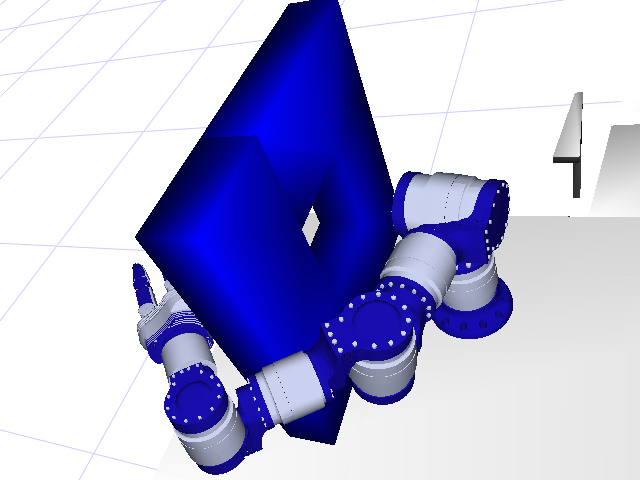
\includegraphics[width=0.4\textwidth]{figures/targetPosition.png} 	
	       \label{fig:IntroductionTargetPosition}
          }
		  \subfigure[Possible Paths]{
		   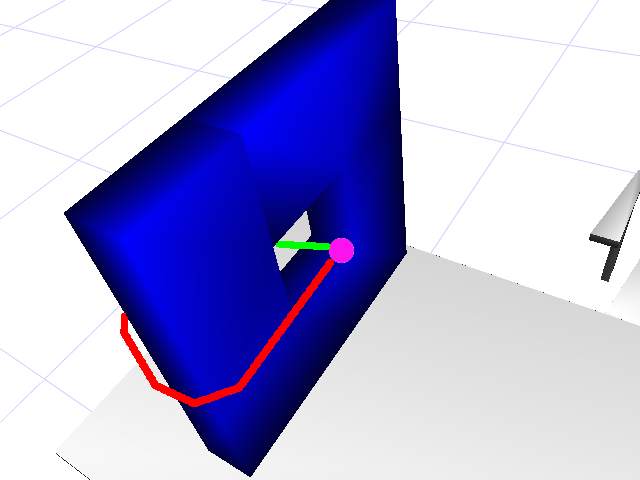
\includegraphics[width=0.4\textwidth]{figures/Torus3DEndingPointsDrawn.png} 
		   \label{fig:IntroductionPaths}
          }          
          \caption{Application example: An optimal planner would find the green path, however the red one would be more useful}
          \label{fig:Introduction1}
\end{figure}


%%%%%%%%%%%%%%%%%%%%%%%%%%%%%%%%%%%%%%%%%%%%%%%%%%%%%%%%%%%%%%%%
\section{Related Work}
\label{sec:RelatedWork}
Here we can cite work of Likhachev et al \cite{Bhattacharya2011Homotopy3D}, and stuff about Distance Transform such as the work of Pedro Fzelnzab as well as the application of Distance Transforms to Path Planning, although its goal was different than ours

Mention coverage stuff by Zelinsky \cite{Zelinsky1993Coverage}

%%%%%%%%%%%%%%%%%%%%%%%%%%%%%%%%%%%%%%%%%%%%%%%%%%%%%%%%%%%%%%%%
\subsection{Homotopy classes}

% -----------------------------------------------
\label{subsec:HomotopyClasses}

% .....................................................
\subsubsection{Homotopy in 2D spaces}
Problem pretty much solved by Stilman \cite{Igarashi2010Homotopy2D} and Likhachev \cite{Bhattacharya2010Homotopy2D}

% .....................................................
\subsubsection{Homotopy in 3D spaces}
Why it is hard and recent stuff from Knepper \cite{Knepper2012Equivalence} and roots from Simeon \cite{Simeon2000VisibilityPRM} and Jaillet \cite{Jaillet2008PathDeformation}

%%%%%%%%%%%%%%%%%%%%%%%%%%%%%%%%%%%%%%%%%%%%%%%%%%%%%%%%
\section{Definitions}
\label{sec:Definitions}


% ..............................................
% Discrete  Connected Space
\begin{definition}[Discrete Connected Space - DCS]
Let $\Omega$ be a finite closed subspace of $\Z^{n}$ composed by a finite number of nodes $n_{i}$. We define that $\Omega$ is \emph{discrete} and \emph{connected} if for any two nodes $n_{i}$ and $n_{j}$ we can always find a path between both of them.     
\end{definition}

Examples of a DCS can be a uniformly gridded box as shown in \ref{fig:PathConnectedSet} or a more complex space such as \ref{fig:ConnectedSet}. For both figures, consider that the DCS is the space enclosed by the colored grids. In this paper we will focus mostly in DCS $\in \Z^{3}$ although the concept is general for other dimensions.

\begin{figure}[]
		\centering
		  \subfigure[Path Connected Set]{
		   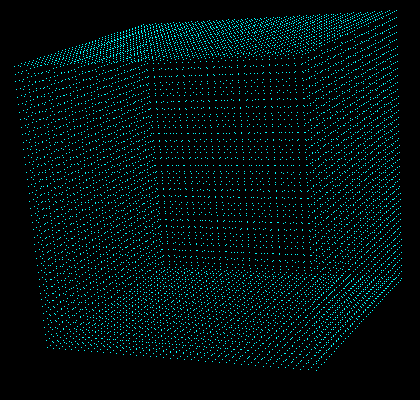
\includegraphics[width=0.4\textwidth]{figures/PathConnectedSet.png} 
		   \label{fig:PathConnectedSet}
          }
          \subfigure[Connected Set]{
	       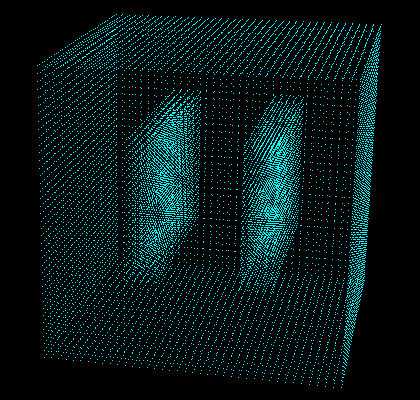
\includegraphics[width=0.4\textwidth]{figures/ConnectedSet.png} 	
	       \label{fig:ConnectedSet}
          }
          \caption{Examples of Discrete Connected Sets}
          \label{fig:DiscreteSets}
\end{figure}

% ................................................
% Set Distance Definition
\begin{definition}[Set Distance]
Let $\Omega$ be a \emph{discrete connected space}. We define a binary function \textsl{F}:
\begin{center}
$ \textsl{F} : \Omega \rightarrow \{0,1 \} $
\end{center}
From the definition above, we further define the subset $\mathcal{P}$ as the collection of nodes $n_{i} \in \Omega$ such that:

\begin{equation}
\PathSet = \{ n_{i} \in \DCS | \textsl{F}(n_{i}) = 0 \}
\end{equation}

The \emph{set distance} of a node $n_{i}$ with respect to $\PathSet$ is defined as:
\begin{equation}
 \textsl{D}_{\PathSet}(n_{i}) = \min_{p \in \PathSet}{ d(n_{i},p) } 
\end{equation}

where $d(n_{i}, p)$ is some measure of the distance between $n_{i}$ and $p$. 
\end{definition}

A special case of a set distance is the well-known concept of \emph{ Distance transform} (\cite{Fabbri2008Survey2DEDT},\cite{Jones2006Survey3DDT}). In this case, the set \PathSet is composed of the nodes occupied by the objects. Furthermore, the metric $d$ is generally taken as the Euclidean distance given by:

\[ d(n_{i}, p) = \sqrt[]{ ( {n_{i}}_{x} - p_{x})^{2} + ({n_{i}}_{y} - p_{y})^{2} + ({n_{i}}_{z} - p_{z})^{2} } \]

when $\Omega \in \Z^{3}$. Since $\Omega$ is not necessarily a \emph{path-connected space}, we cannot use the EDT as metric. An intuitive metric would be the shortest path from node $n_{i}$ to $p$.

% ............................................
% Path Set Distance Definition
\begin{definition}[Path Set Distance]
Let \PathSet be a set defined by a function $F$ evaluated on a discrete connected space $\Omega$. Consider a path $\Path \in \Omega$. We define the \emph{Path Set Distance}(\PathSetDistance) of \Path with respect to \PathSet as: 

\begin{equation}
\PathSetDistance(\Path) = \min \sum_{i = 1}^{k} \textsl{D}_{\PathSet}(n_{i})
\end{equation} 

where $n_{i} \in P, i = \{1,2,...,k\}$
\end{definition}

% ..............................................
% Path Distance
\begin{definition}
Consider two paths $\Path_{A}$ and $\Path_{B}$ $\in \DCS$. We define \emph{Path Distance} as the \emph{set distance} of $\Path_{A}$ with respect to the set formed by the nodes of $\Path_{B}$ (or viceversa). Formally:

\begin{equation}
\PathDistance(\Path_{A}, \Path_{B}) = \SetDistance_{P_{A}}(P_{B})
\end{equation}
\end{definition}

% ................................................
% Bounded Diverse Path Problem
\begin{definition}
Given a \emph{DCS} $\DCS$ and a set of paths $\PathSet = {\Path_{1}, \Path_{2},...\Path_{M}}$ 
\end{definition}

\bibliographystyle{plain}
\bibliography{references}

\end{document}
